\section{Milestone I}\label{M1}
In this section we want to study the evolution of the uniform background in the Universe. Our main goal of this section will be to implement methods that computes the Hubble parameter, as well as related time- and distance measures \note{Rewrite}. To do this, we will solve \note{simple} ordinary differential equations (ODEs) numerically. For the fiducial cosmology we will use results from \cite{Planck2020}. We will then test our implementation with known theoretical solutions, to assess the validity of our methods. 

The main goal of this section is mainly concerned with using known parameter values to \note{predict/solve} the background cosmology. Another interesting aspect is to use data to constrain such cosmological parameters. To do this, we will use data from supernova observations \cite{Supernova2014Betoule}, containing luminosity distance associated with different values of redshift. Implementing our solver, we will implement a simple Markov chain Monte Carlo (MCMC) algorithm, in order to estimate the best fits of $h,\,\Omega_m$ and $\Omega_\Lambda$, which are the Hubble parameter, and the density parameter of matter and dark energy, respectively.   


\subsection{Theory}\label{M1:theory}
The theory behind this milestone. \note{Define ALL parameters}

\note{Neutrinos are on the loose. Catch them before it's too late.}

\note{Define Omegas.}

When we don't assume $k=0$ the Friedmann equation can be written as 
\begin{equation}
    H = H_0 \sqrt{\omn a^{-3} + \oradn a^{-4} + \okn a^{-2} + \oln}, \label{eq:M1:theory:Friedmann_H_omegas}
\end{equation}
where $H\equiv\dot{a}/a$ is the Hubble parameter, where the dot denotes a derivative with respect to cosmic time, $t$. For brevity, we have expressed the density parameters of matter and radiation as $\omn=\obn+\ocdmn$ and $\oradn=\ogn+\onun$, respectively. The density parameters of radiation follow from the CMB temperature, and are given by 
\begin{align}
    \ogn &= 2 \cdot \frac{\pi^2}{30} \frac{(k_b T_\mathrm{CMB0})^4}{\hbar^3 c^5} \cdot \frac{8\pi G}{3H_0^2}, \label{eq:M1:theory:omega_gamma0_T} \\
    \onun &= N_\mathrm{eff} \cdot \frac{7}{8} \cdot \closed{\frac{4}{11}}^{4/3} \ogn. \label{eq:M1:theory:omega_nu0_T}
\end{align}
%
We also introduce the scaled Hubble factor, $\H\equiv aH$. Rather than working with the scale factor, $a(t)$, we will mainly be working with the logarithm of the scale factor 
\begin{equation} \label{eq:M1:theory:x_dx_definitions}
    x\equiv \ln a,\quad '\equiv \dv{x}. 
\end{equation}
%
%
The resulting expression for $\Hx$ is thus  
\begin{equation} \label{eq:M1:theory:Hp_of_x}
    \Hx = H_0 \sqrt{\omn e^{-x} + \oradn e^{-2x} + \okn + \oln e^{2x}}. 
\end{equation}
%
%
We will need the first and second derivative of $\Hx$. To simplify the resulting expressions, we define the function, $g(x)$, as the derivative of the term inside the square root in Eq. \eqref{eq:M1:theory:Hp_of_x}, namely 
\begin{equation}
    g(x) \equiv -\omn e^{-x} -2\oradn e^{-2x} + 2\oln e^{2x}. \label{eq:M1:theory:g_of_x} 
\end{equation} 
%
Using the chain rule, the first two derivatives of $\Hx$ can be written as 
\begin{align} 
    \dv{\H(x)}{x} &= \frac{H_0^2}{2\Hx}g(x), \label{eq:M1:theory:dHp_dx} \\
    \dv[2]{\Hx}{x} &= \frac{H_0^2}{2\Hx}\bracket{g'(x) - \frac{1}{2}\closed{\frac{H_0 g(x)}{\Hx}}^2}. \label{eq:M1:theory:ddHp_ddx}
\end{align}
%
One of the main time variables we will be working with is the conformal time, $\eta$. In terms of $x$ and $\H$, we have the following differential equation 
\begin{equation}
    \dv{\eta}{x} = \frac{c}{\H}. \label{eq:M1:theory:deta_dx}
\end{equation}
Numerically, this can be solved by integrating. 
\begin{equation}
    \eta(x) = \int_{-\infty}^{x'} \frac{c\,\dd x'}{\H(x')}. \label{eq:M1:theory:eta_of_x_integral_expression}
\end{equation}
%
The initial condition we have is $\eta(-\infty)=0$. Noting from Eq. \eqref{eq:M1:theory:Hp_of_x} that $\Hx\to H_0\sqrt{\oradn}e^{-x}$ as $x\to-\infty$, we get an analytical approximation for the initial condition of $\eta$ at early times 
\begin{align}
    \eta(x_\mathrm{start}) \approx \int_{-\infty}^{x_\mathrm{start}} \frac{c\,\dd x'}{H_0\sqrt{\oradn}} e^{x'} = \frac{c}{\H(x_\mathrm{start})}. \label{eq:M1:theory:eta_of_xstart_analytical_approximation}
\end{align} 
%

For the supernova fitting, we will need a measure of the luminosity distance, $d_L$, defined as 
\begin{equation}
    d_L(a) = \frac{d_A}{a^2} = \frac{r}{a}, \label{eq:m1:theory:dL_of_a_general expression}
\end{equation} 
where $d_A=ar$ is the angular distance, expressed in terms of the co-moving distance, $r$. Photons move on $0$-geodesics, and from the line-element in spherical coordinates,
\begin{equation}
    ds^2 = -c^2 dt^2 + a^2 \closed{\frac{dr^2}{1-kr^2} + r^2 d\theta^2 + r^2 \sin^2\theta d\phi^2}, \label{eq:M1:theory:FLRW_general_nonflat_spherical}
\end{equation} 
we get the co-moving distance by integrating the line element of radially moving photons. For a photon emitted at, $(t,r)$, reaching an observer at $(t_0, 0)$, we get 
\begin{equation}
    \int_0^r \frac{\dd r'}{\sqrt{1-k r'}} = \int_t^{t_0} \frac{c\,\dd t}{a}\equiv\chi. \label{eq:M1:theory:chi_integral_expression}
\end{equation} 
$\chi$ is closely related to the conformal time, as seen by manipulating the RHS of Eq. \eqref{eq:M1:theory:chi_integral_expression}, yielding  
\begin{equation}
    \chi = \int_t^{t_0} \frac{c\,\dd t}{a} = \int_x^0 \frac{c\,\dd x'}{\H(x')} = \eta(0) - \eta(x). \label{eq:M1:theory:chi_eta0_minus_eta_of_x}
\end{equation}
The LHS of Eq. \eqref{eq:M1:theory:chi_integral_expression} can be solved for $r$, giving 
\begin{equation}
    r = \begin{cases}
        \chi\cdot \frac{\sin\closed{\sqrt{\abs{\okn}} H_0 \chi / c}}{\closed{\sqrt{\abs{\okn}} H_0 \chi / c}},\quad &\okn < 0 \\ 
        \chi,\quad &\okn=0 \\ 
        \chi\cdot \frac{\sinh\closed{\sqrt{\abs{\okn}} H_0 \chi / c}}{\closed{\sqrt{\abs{\okn}} H_0 \chi / c}},\quad &\okn > 0
    \end{cases}
\end{equation} 

%
\begin{align}
    \ok(x) &= \frac{\okn}{\Hx^2 / H_0^2}, \\ 
    \om(x) &= \frac{\omn}{e^x \Hx^2 / H_0^2}, \\ 
    \og(x) &= \frac{\ogn}{e^{2x} \Hx^2 / H_0^2}, \\ 
    \ol(x) &= \frac{\oln}{e^{-2x} \Hx^2 / H_0^2},     
\end{align}
%




The density parameter of the photons today, $\ogn$, is given by 
\begin{equation}
    \ogn = 2 \cdot \frac{\pi^2}{30} \frac{(k_b T_\mathrm{CMB0})^4}{\hbar^3 c^5} \cdot \frac{8\pi G}{3H_0^2}, \label{eq:M1:theory:omega_gamma0_Told}
\end{equation}
where $T_\mathrm{CMB0}$ denotes the temperature of the CMB today. 


\subsection{Implementation details}\label{M1:implementation} 
Something about the numerical work.

\subsection{Results}\label{M1:results}
\subsubsection{Sanity checks}
Show and discuss the results.



\begin{figure}
    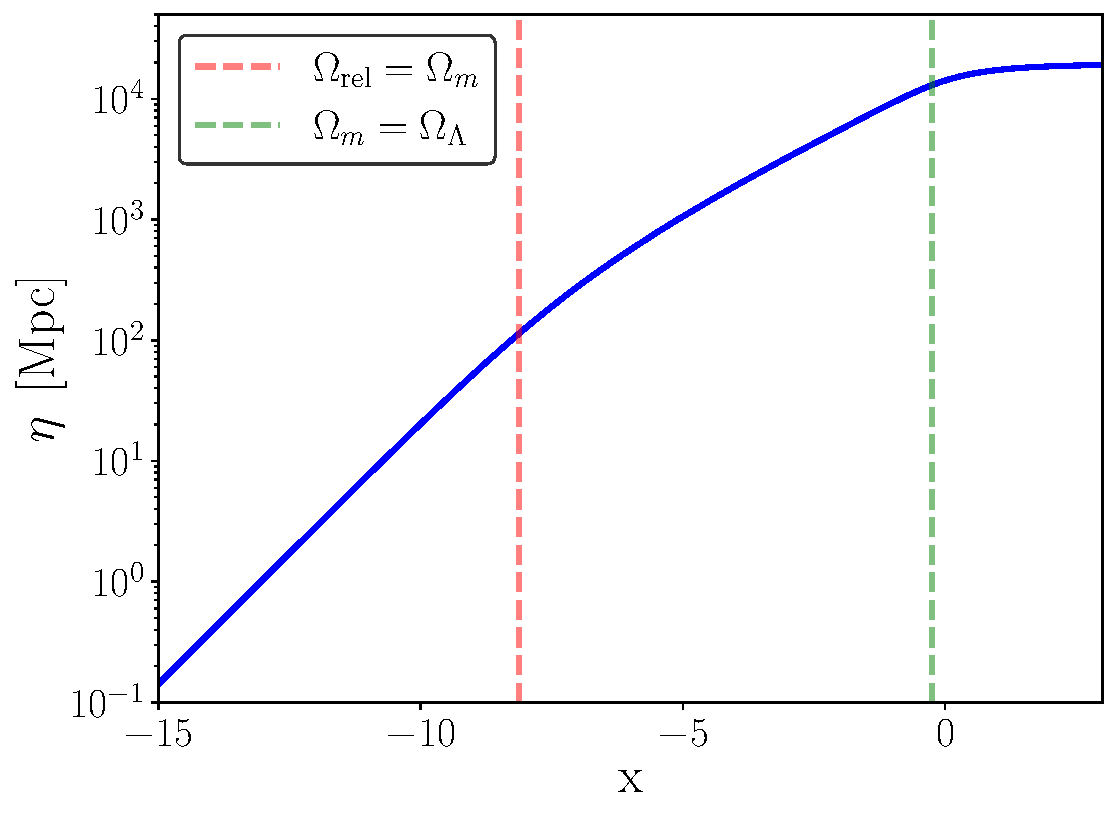
\includegraphics[width=\linewidth]{compare_eta.pdf}
    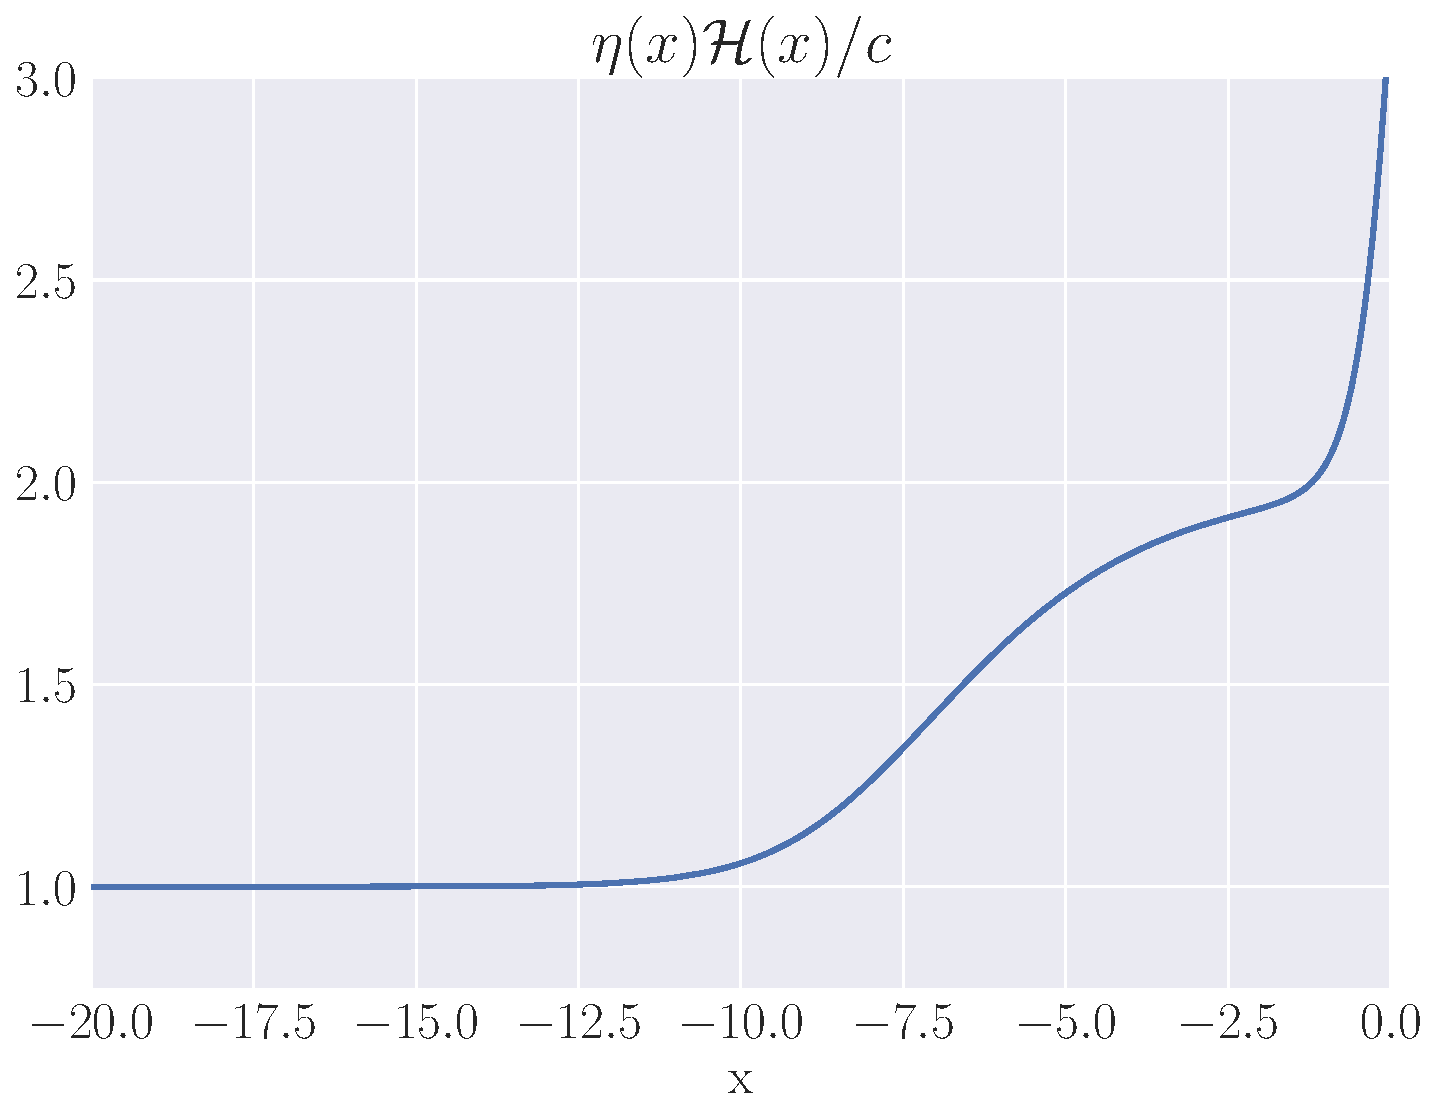
\includegraphics[width=\linewidth]{compare_eta_H_over_c.pdf}
    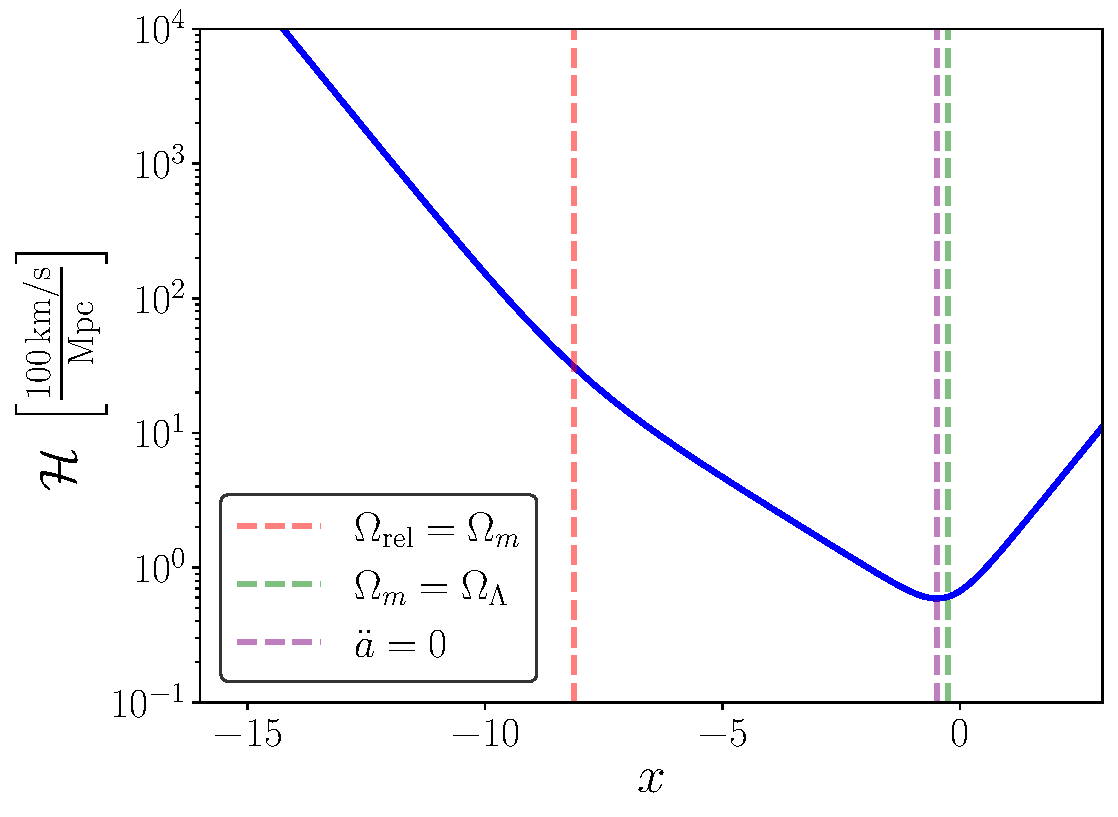
\includegraphics[width=\linewidth]{compare_Hp.pdf}
\end{figure}

\begin{figure}[ht!]
    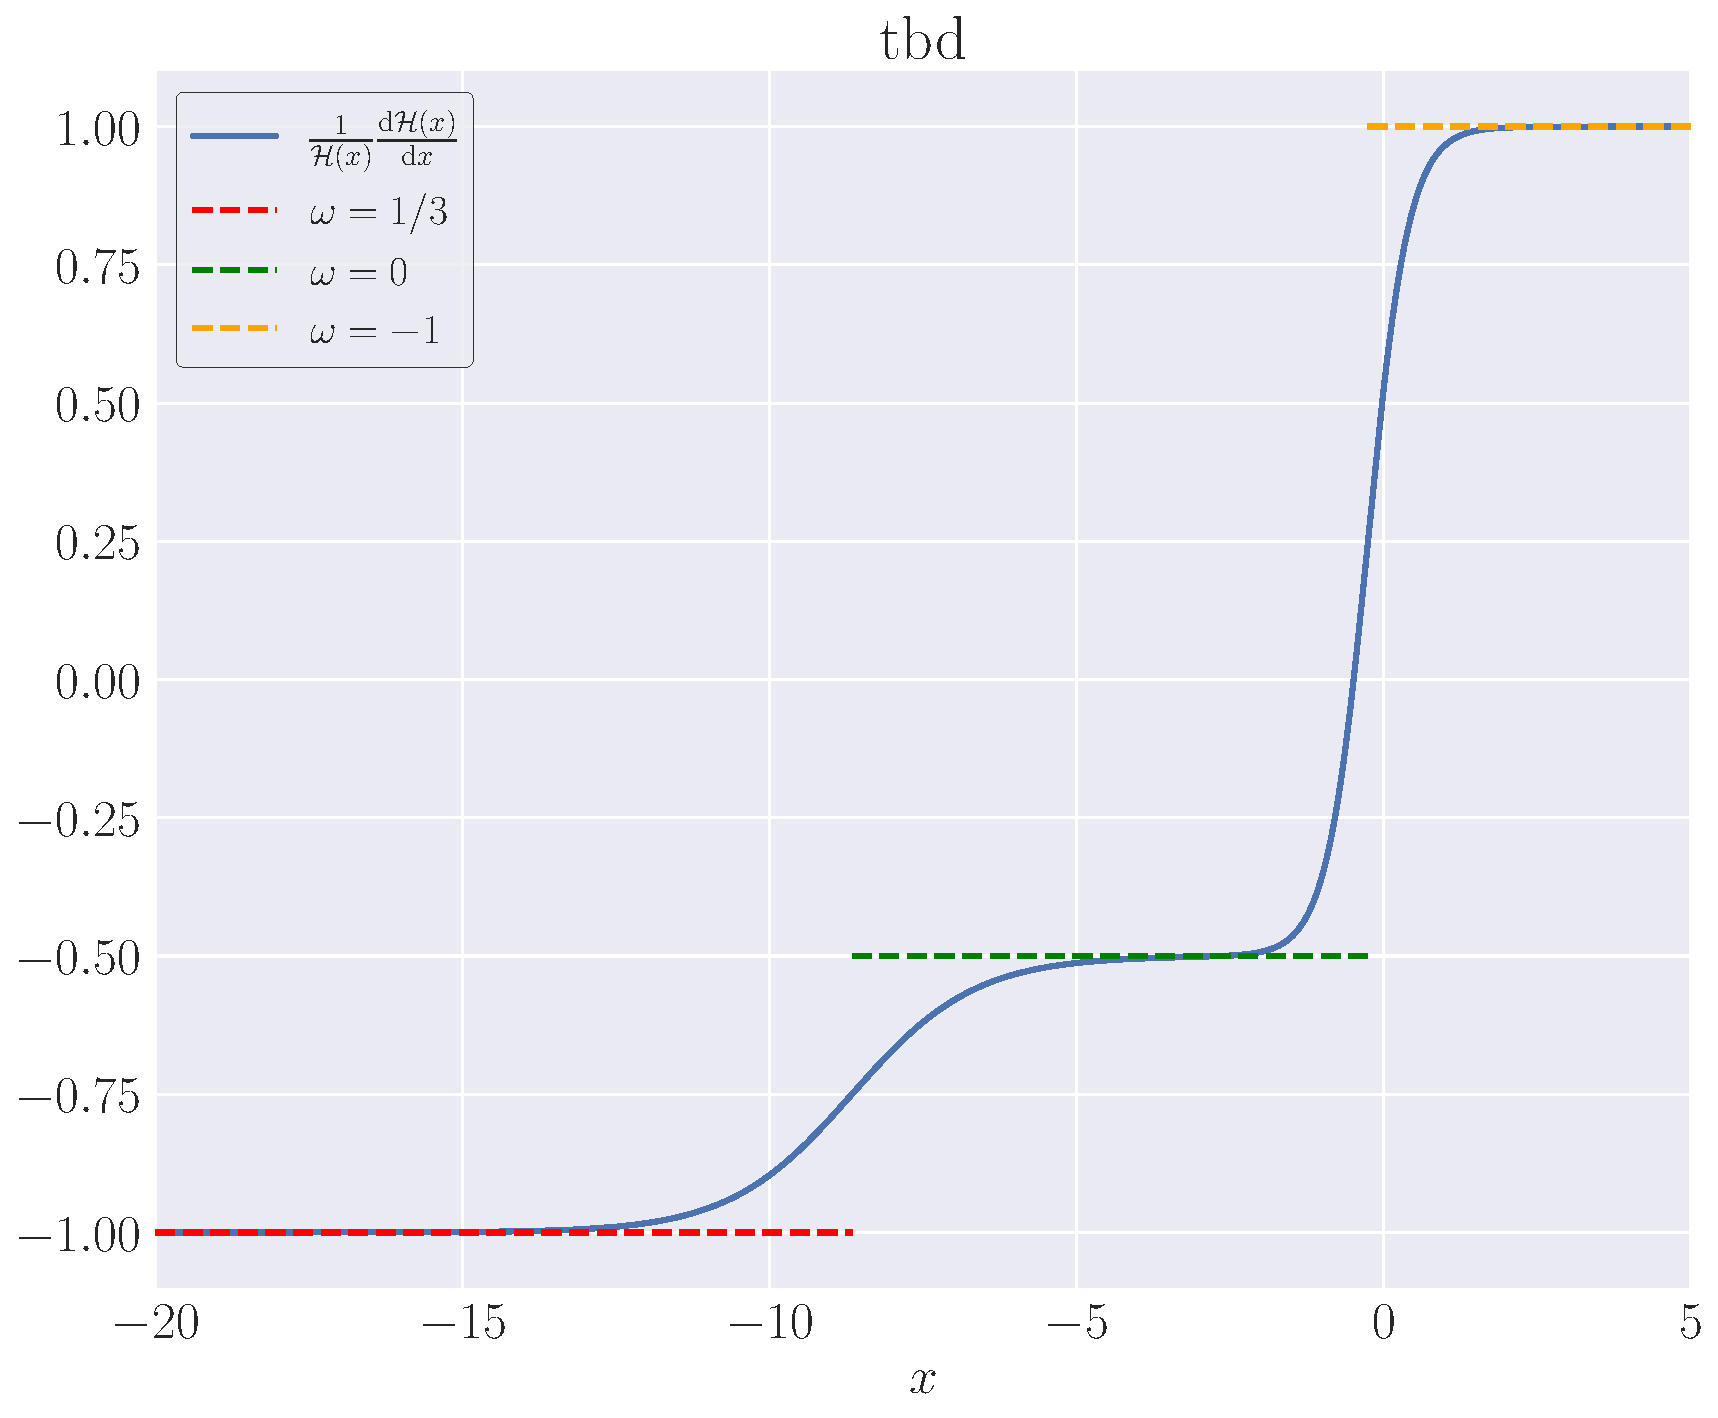
\includegraphics[width=\linewidth]{dH_over_H.pdf}
    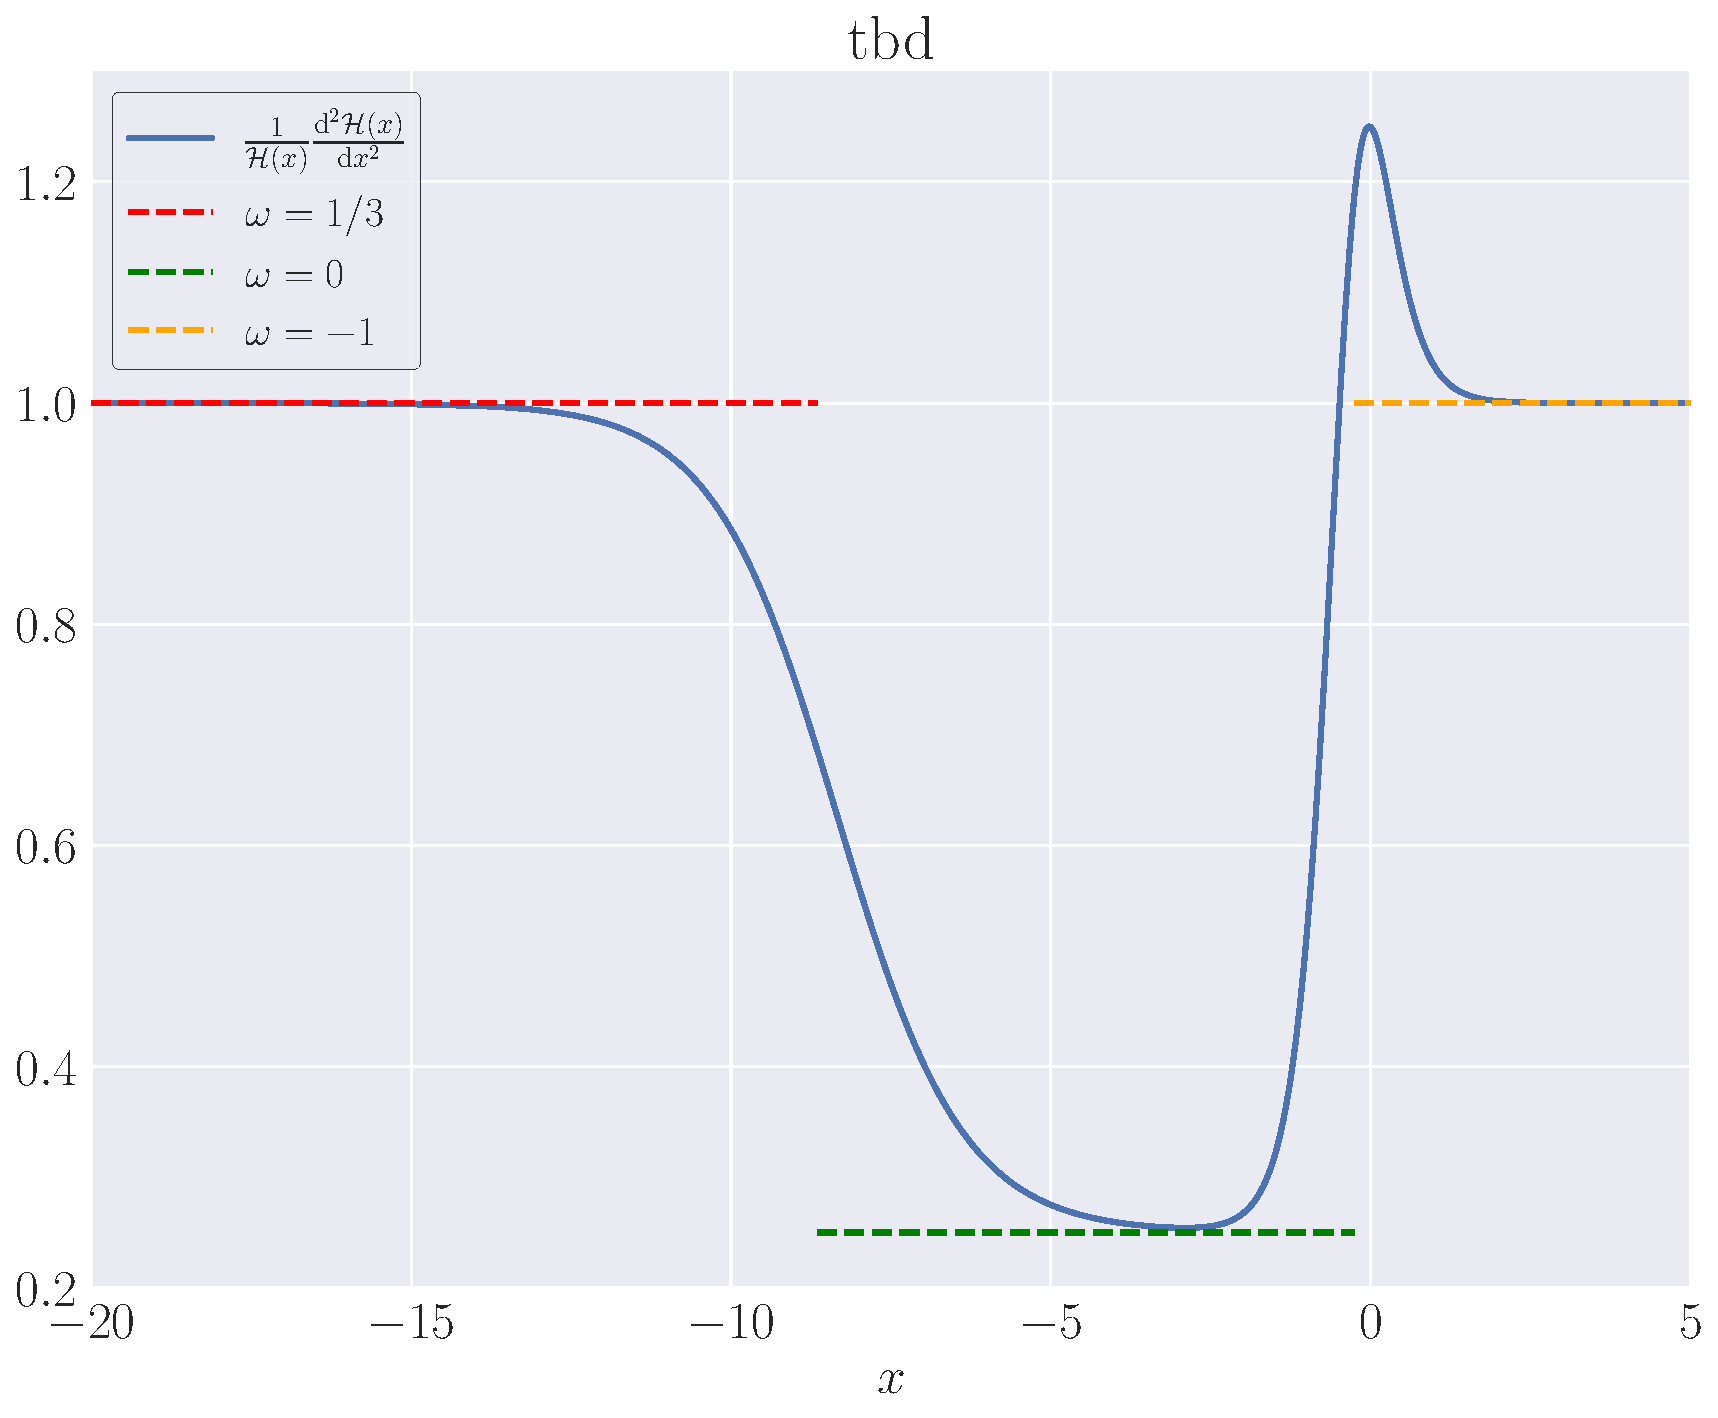
\includegraphics[width=\linewidth]{ddH_over_H.pdf}
\end{figure}

\begin{figure}[ht!]
    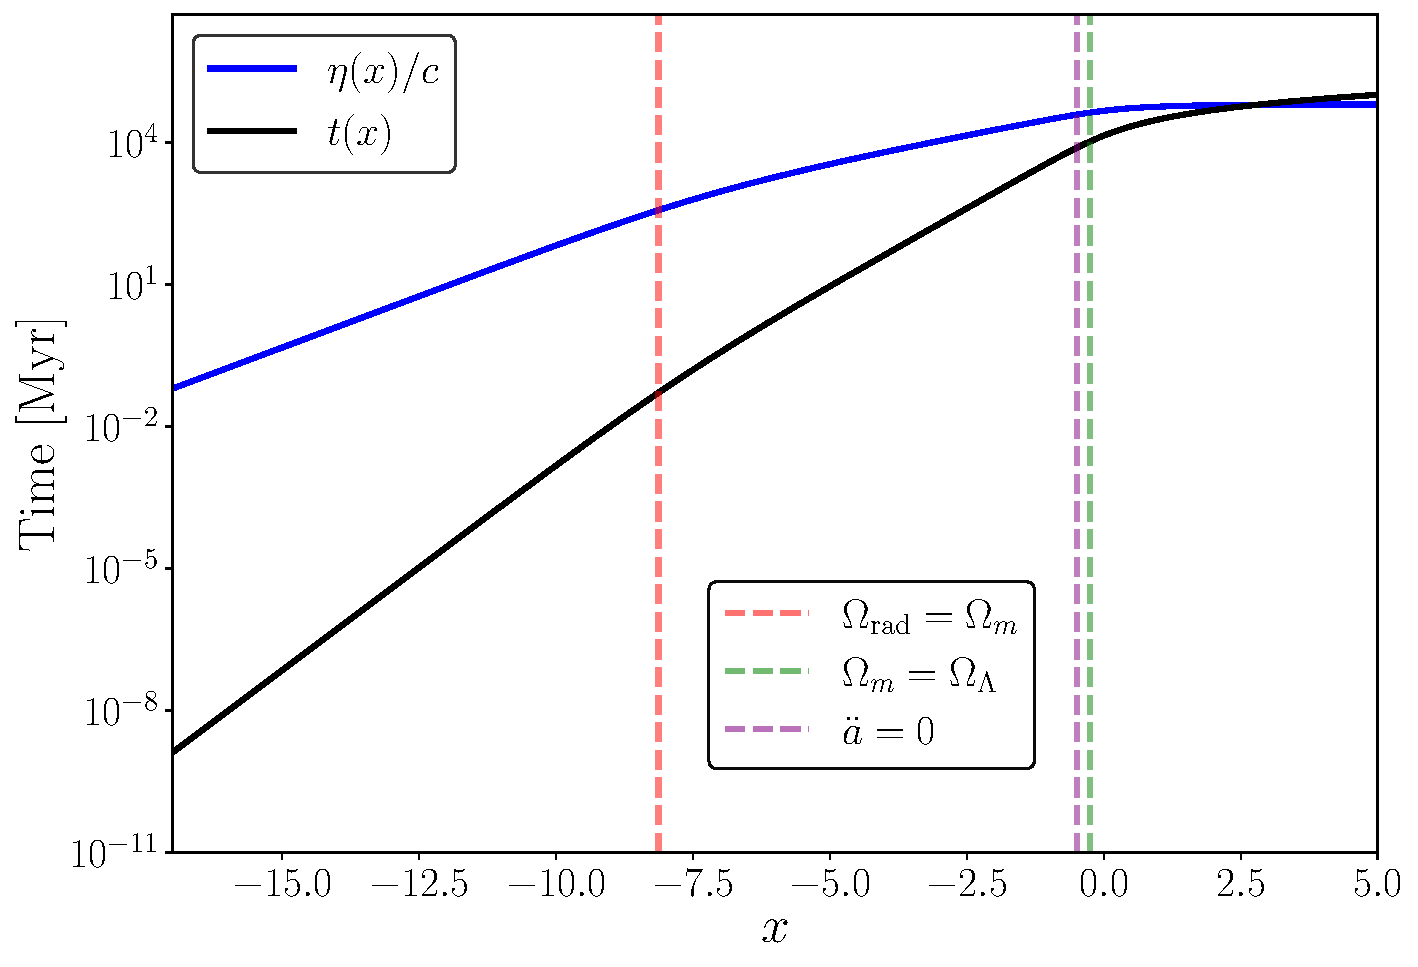
\includegraphics[width=\linewidth]{t_and_eta_c.pdf}
\end{figure}


\begin{figure}[ht!]
    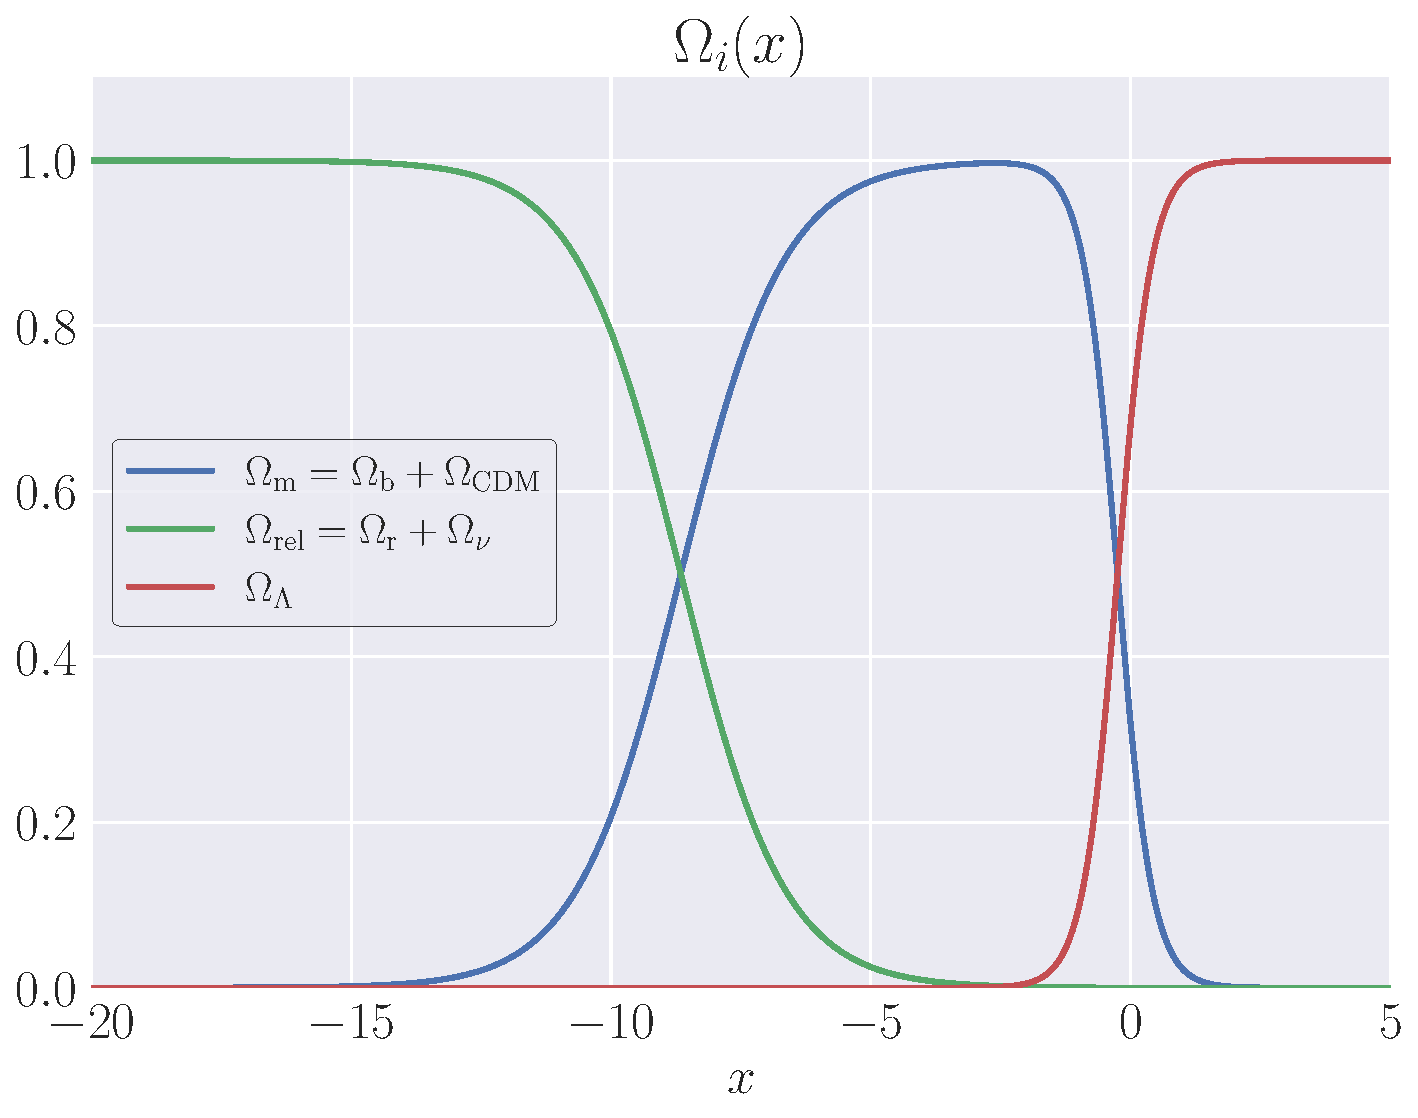
\includegraphics[width=\linewidth]{omega_i_of_x.pdf}
\end{figure}

\begin{figure}[ht!]
    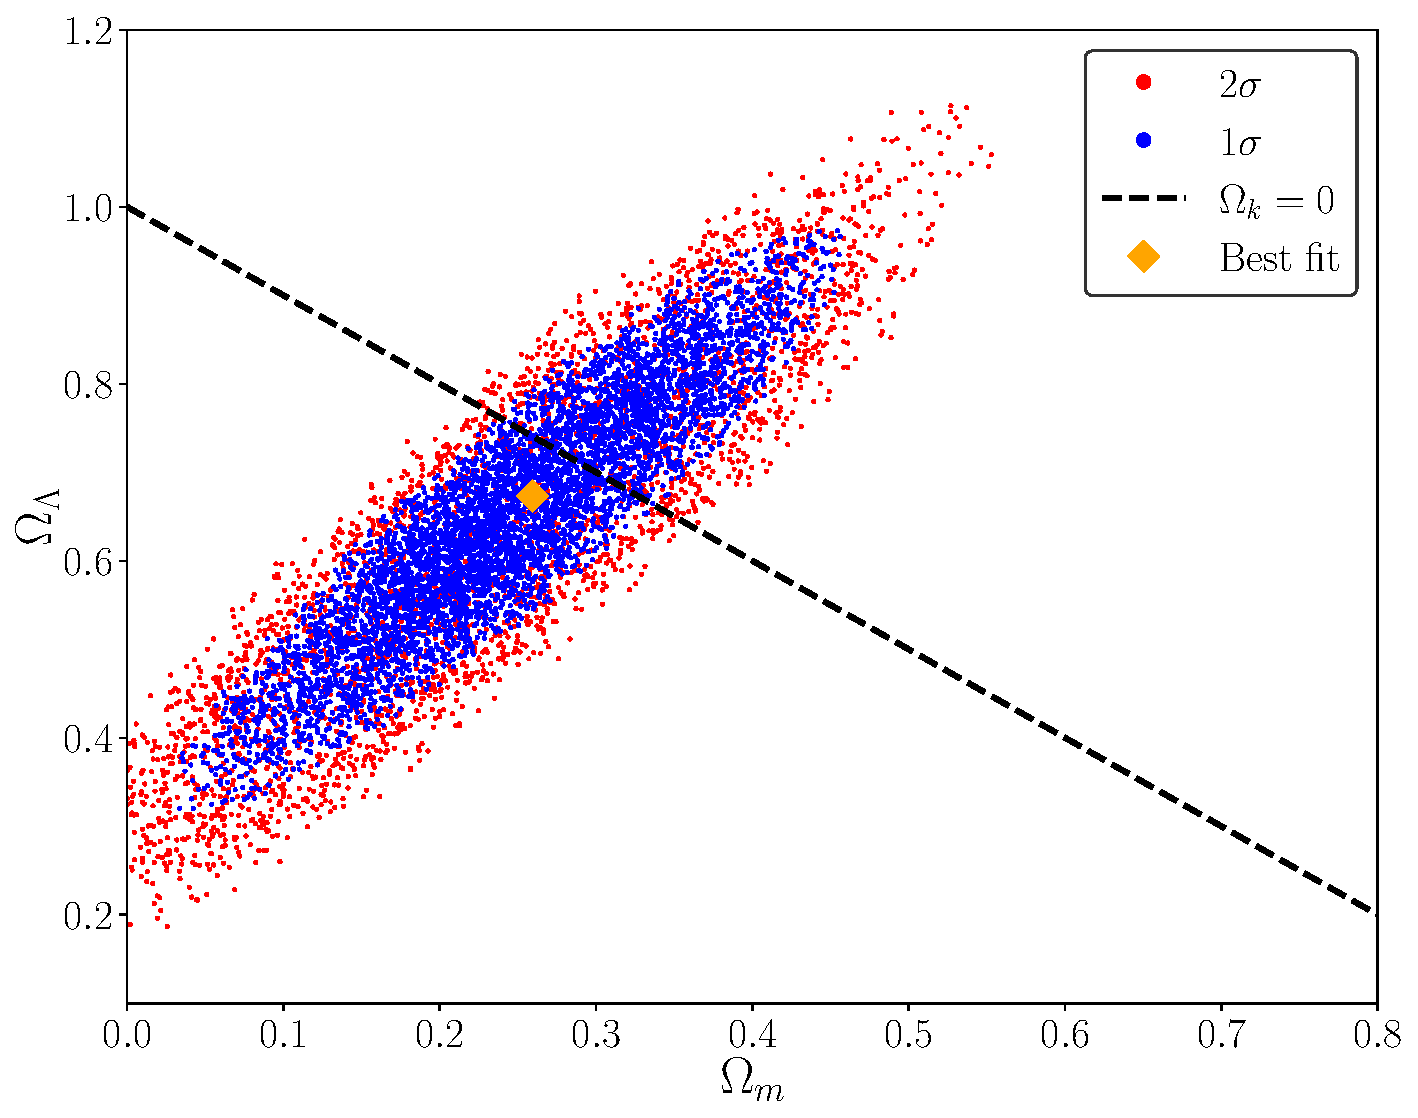
\includegraphics[width=\linewidth]{mcmc_supernova_fit_Nburn1000.pdf}
    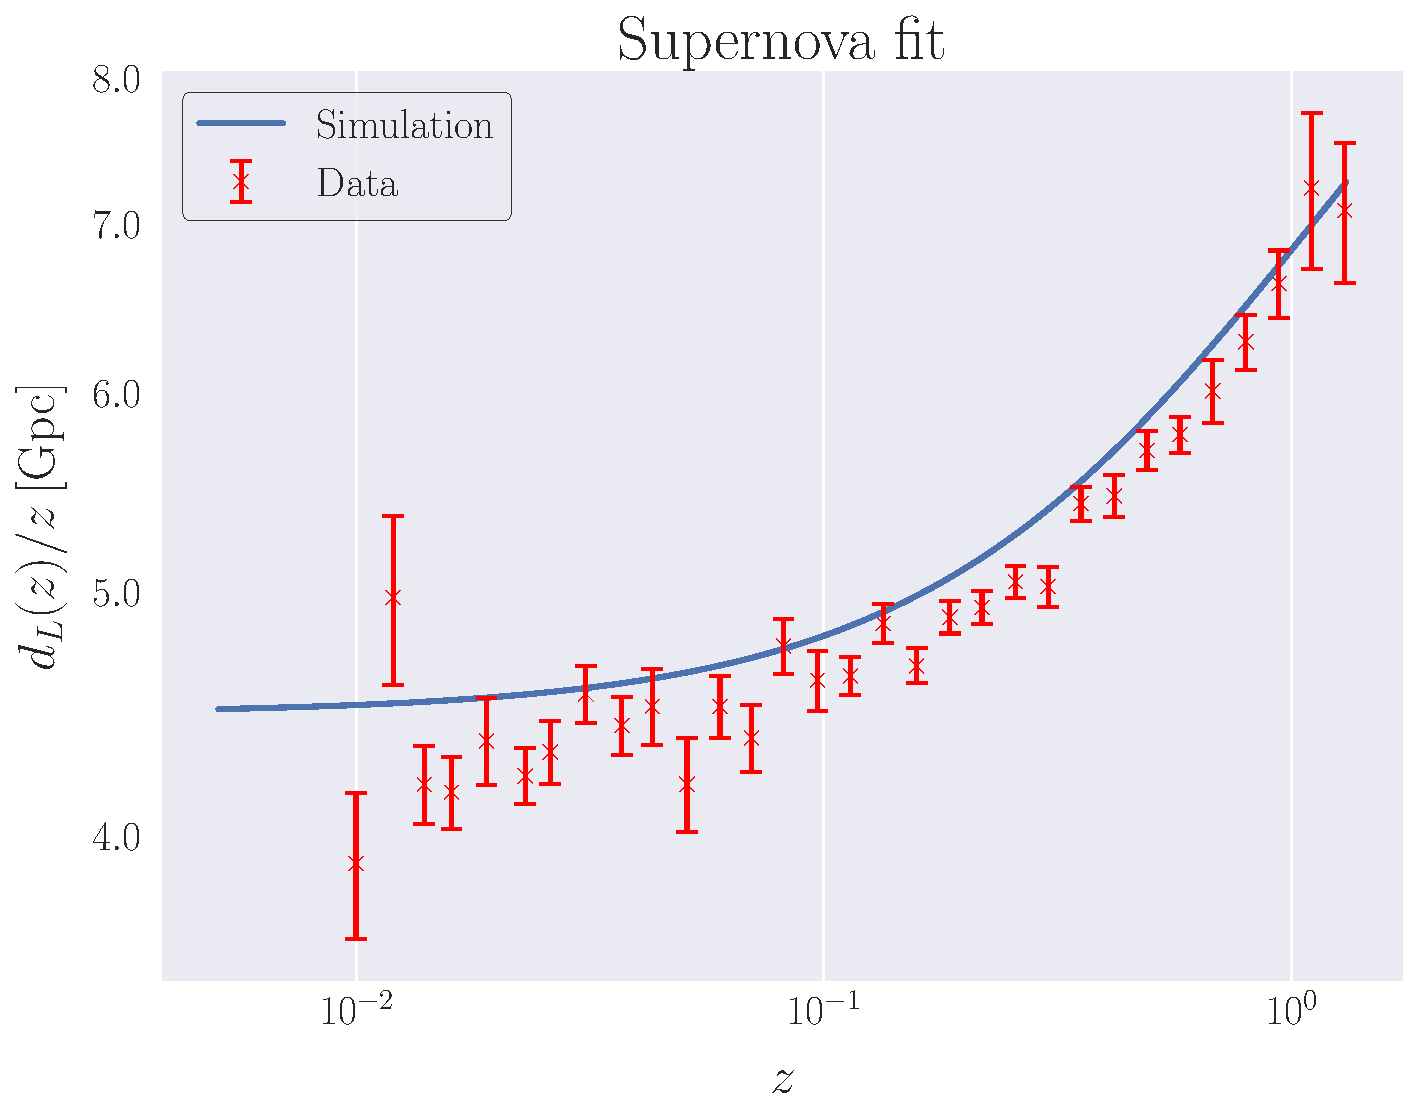
\includegraphics[width=\linewidth]{dL_z_compare_log.pdf}
\end{figure}

\begin{figure}[ht!]
    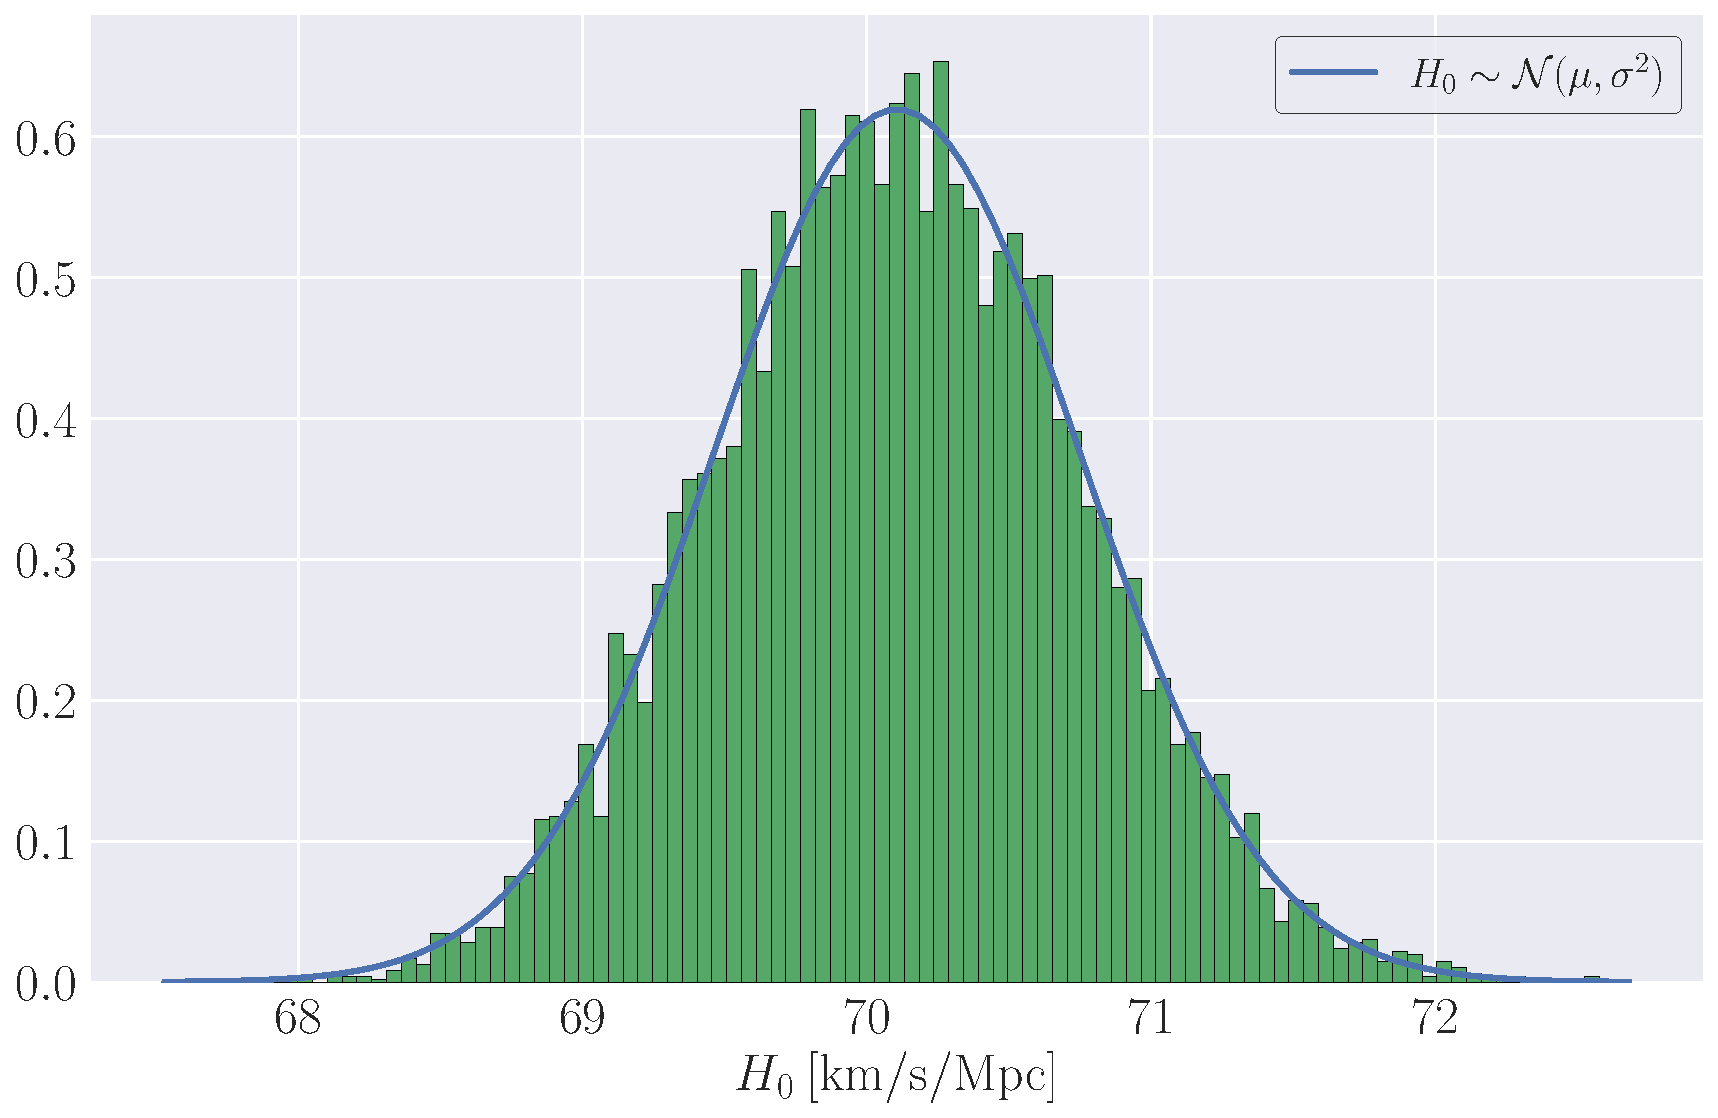
\includegraphics[width=\linewidth]{H0_pdf_Nburn1000.pdf}    
\end{figure}